
\subsubsection{Physical Test}
An additional small test will be run as an informal experiment to see whether what has been 
learned by the RL agents can be implemented in real-life applications. That is why an attempt 
will be made to deploy the best working model on a physical drone. The details of this test 
will shortly be discussed here.

This will be implemented using a drone that is primarily comprised of a quadcopter with 
telemetry controlled propellers and a Raspberry Pi on which the model will be running.
The drone used is the RDDRONE-FMUK66 model, as seen in Figure \ref{Drone}.
This device is a lightweight version of a drone that needs to be assembled component 
by component making it easily modifiable. Important 
to note, is the fact that the drone comes with the availability of controlling the 
drone using a high-level API called PixHawk. As has been mentioned before, there is easy 
transferability of the relevant control systems since AirSim also is compatible with 
PixHawk, making this part of the deployment much smoother. 

\begin{Figure}
    \centering
    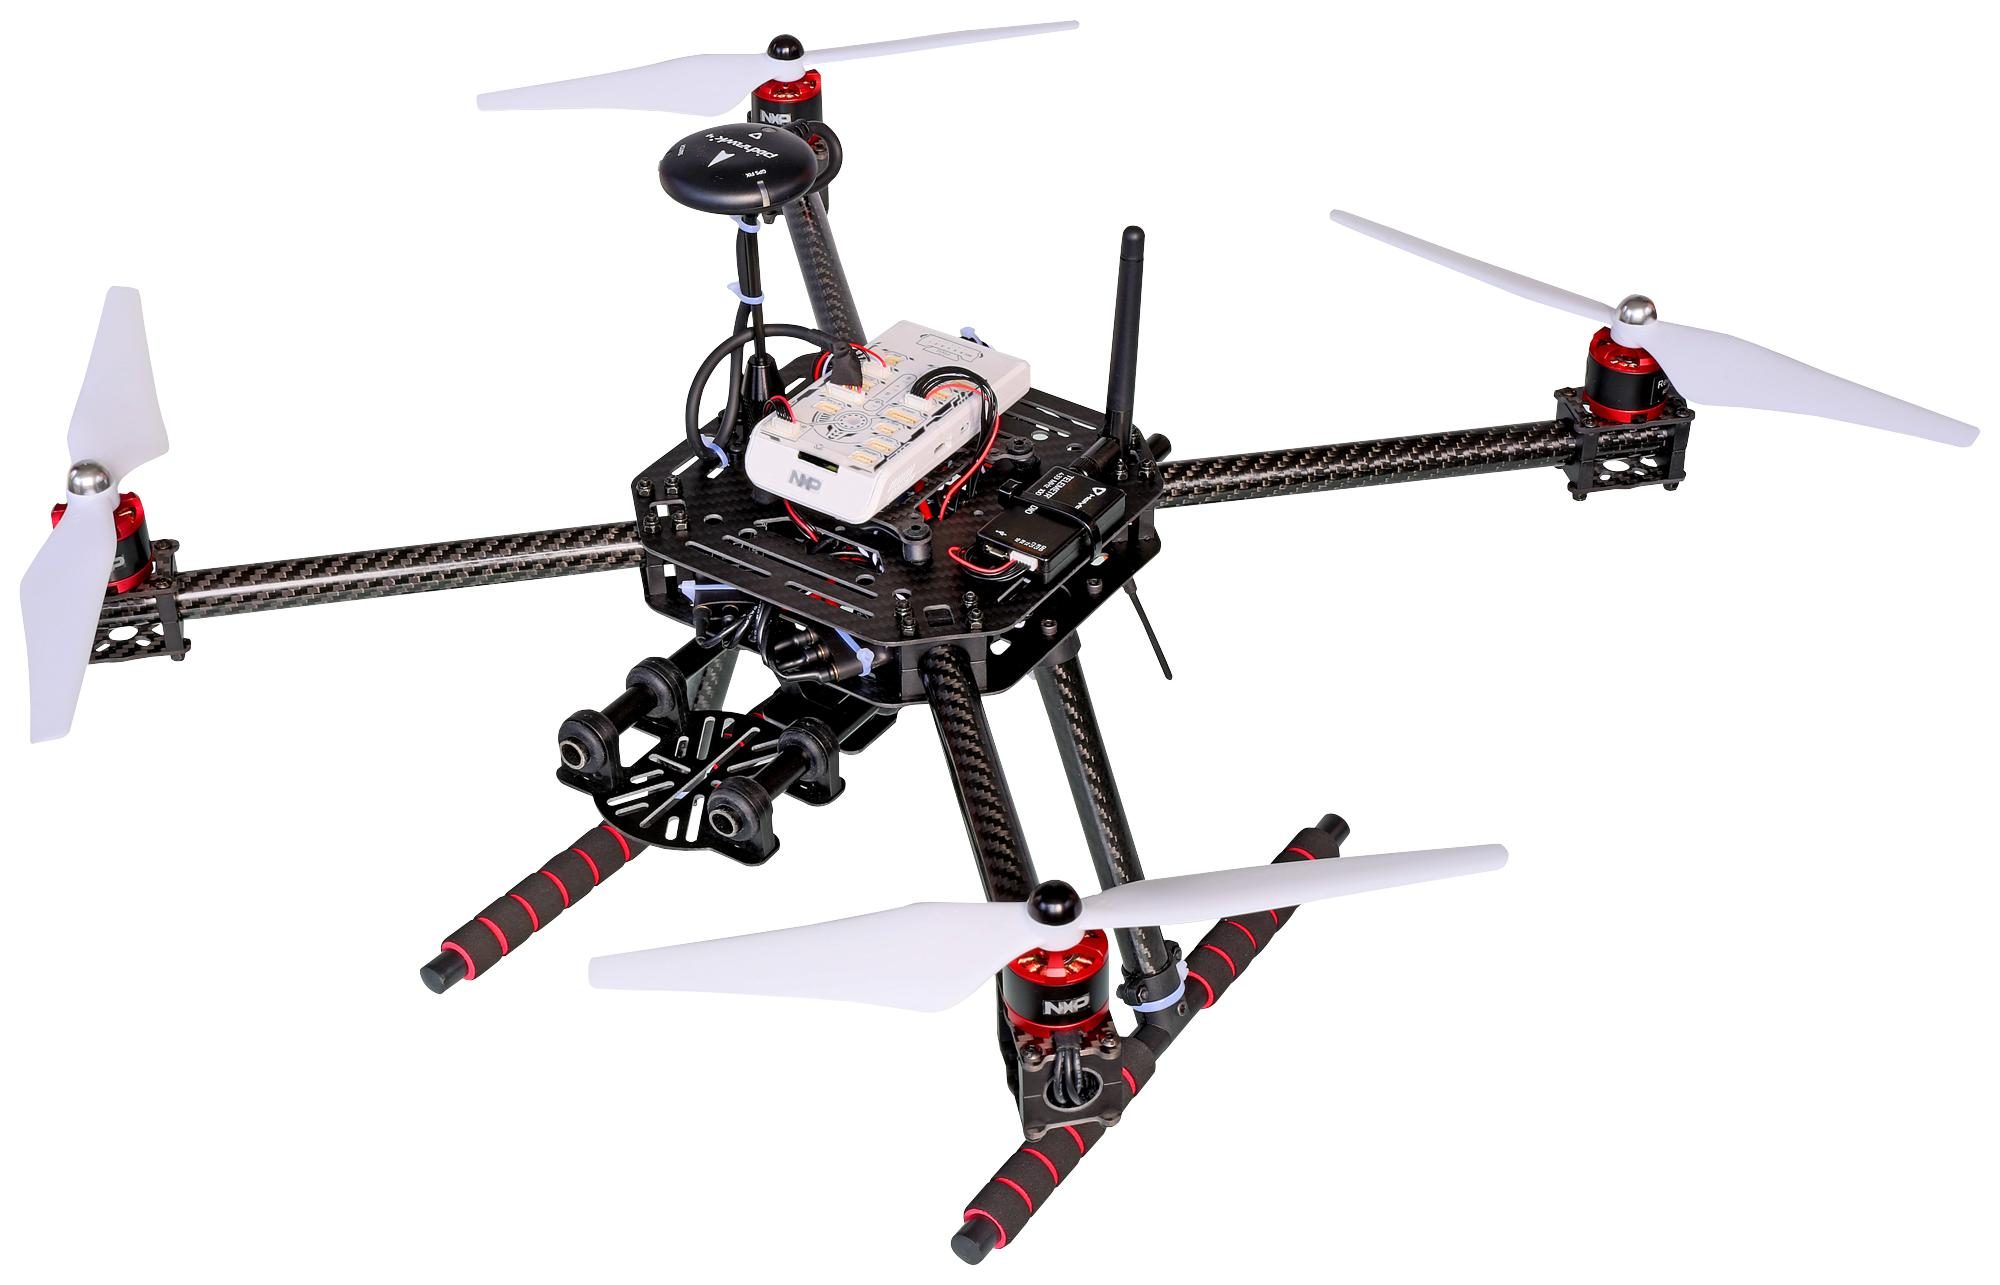
\includegraphics[width=0.6\linewidth]{methods/drone.jpg}
    \captionof{figure}{The RDDRONE-FMUK66 drone }
    \label{Drone}
\end{Figure}

The Raspberry Pi (RP) 4B contain 4GB of RAM, with which it will have to perform the behavior
required. This behavior will comprise of two aspects. First, the RL agent which will simply 
be the trained policy that can be used to make decision on the go quite easily. The trained 
networks are small in size, giving the RP the chance to handle this computiational load. However, 
the other aspect, is the lack of a bounding box algorithm. Since the RL agent depends on a bounding 
box as an input to make its decisions on, and this bounding box was provided for with ground truth 
information from the simulation, this becomes a problem for this physical drone. That is why 
there is the need for an object detection algorithm to provide this bounding box. Running an 
object detector that can process the stream of video coming to the RP is not trivial. Most 
object detectors are quite heavy. Luckily there are many advancements in reducing these computational 
requirements lately. One of these efforts is the model YoloFastest \cite{yolofastest}, which 
will be used to solve the problem. 

Furthermore, seeing as a good working model is a model trained on depth imaging, a second 
problem arises. Depth-imaging from computer vision techniques in real-world applications are 
quite complicated and are often not accurate. Currently, the most applicable technique for this 
is the use of stereovision. Using a double camera as a way to use the differences between 
each frame as a means of calculating the distances to objects, this technology could be used 
to create depth-images with. For the RP, there is already a starter kit that includes 
all the necessary hardware and software requirement to create such depth images. This 
kit, the StereoPi \cite{StereoPi}, includes two cameras and additional libraries to 
help with easy connection to the RP. Furthermore, the StereoPi includes a module that 
can additionally perform some computations. This helps remove some load from the 
RP so that the focus can be on performing the object detection and path planning.
The images that this camera will produce, will first be used to calculate a depth-image,
which will then be used as a potential input to the RL agent. 

The goal here will be to informally see how much of the learned behavior is translated to the
real world. 


\subsubsection{Policy Gradients}
Another way of solving the RL problem, is not by determining Q-values, but by directly 
training a policy. This would result in direct mapping from states to actions, without 
the need for $Q$-values. These 
algorithms, called policy gradients, can use a value function to optimize their policy 
parameters, but their action selection does not depend on this function.

Where the Deep Q-Network uses the difference between its predicted $Q$-value and its observed 
$Q$-values as a loss function in order to adapt the network, policy gradients use a different 
method. Instead, the agent directly tries to maximize the average reward of a policy. This is 
done by focussing on the probability of choosing a certain action under the current policy 
that the network employs and its advantage $A_{t}$. This advantage is defined to be the 
how much better this action is over the other possible actions in a particulare state. 
The equation for this can be observed in Equation \ref{eq:policygradientobjective}:

\begin{equation} 
    L^{P G}(\theta)=E_{t}\left[\log \pi_{\theta}\left(a_{t} \mid s_{t}\right) * A_{t}\right]
    \label{eq:policygradientobjective}
\end{equation}

Optimizing this objective function allows the agent to directly create a policy that 
leads to higher rewards, and avoid bad actions. \newline

\noindent
\textbf{Proximal Policy Optimization } \newline
Policy Gradient methods of reinforcement learning 
bring with them many advantages in the form of better convergence properties \cite{policygradients}. 
However, one disadvantage is that during training time, the changes in policy that 
the network makes can be extremely large. Since small changes in the policy network 
parameters can lead to completely different policies, there is a high volatility during 
training time which can sometimes lead to negative policy changes from which the agent 
can not recover from. 

For this reason, the Proximal Policy Optimization method was introduced (PPO) \cite{ppo-paper}. 
This method simply replaces the objective function by a surrogate which incorporates a 
clip on how large the changes in policy can be. As can be seen in Equation \ref{eq:ppo}, 
this formula simply ensures that the change in the policy parameters do not exceed the 
$\epsilon$ parameter, in either direction. 

\begin{equation} 
    L^{C L I P}(\theta)=\hat{\mathbb{E}}_{t}\left[\min \left(L^{P G}(\theta), clip \left(r_{t}(\theta), 1-\epsilon, 1+\epsilon\right) \hat{A}_{t}\right)\right]
    \label{eq:ppo}
\end{equation}

Using this simple addition to the objective function ensures a more stable training process, 
further improving the convergence of the agent.  

\subsubsection{Mean Average Precision}
An important measure with which to compare different object detection models is 
the mean average precision (mAP) \cite{mAP}. This metric is based on the average 
precision (AP) metric. This method uses the precision and recall of the model 
in order to determine how good the model performs. Both these measures look 
at the prediction matrix of a model. This prediction matrix considers 4 classes 
of possible predictions that the model can make. True positives (TP), which is when 
the model predicted a class and this class was correct. False positives (FP), when the 
predicted class was not the same as the ground truth. Vice versa, the same concepts 
apply for rue negatives (TN) and false negatives (FN). What predictions fall under 
which type, depends on the threshold that the confidence values for each predictions 
are set. Since the goal of object detection is to predict a bounding box with the 
correct class, the predicted bounding box can have a certain margin of error. How 
close the model is to the ground truth before it is considered a correct prediction, 
is measured using the Intersection over Union (IoU):

\begin{equation}
    IoU = \frac{Area of Overlap}{Area of Union}
\end{equation}

Setting a threshold for how large this number is in order to be considered a 
correct classification, can have different effects on the prediction matrix. 
With this information, we can calculate the precision using: 

\begin{equation}
    Precision = \frac{TP}{TP + FP}
\end{equation}.

This can be intuitively explained as the amount of times that a correct prediction 
has been made out of all predictions. Next to this, the recall of a model is defined as 

\begin{equation}
    Recall = \frac{TP}{TP + FN}
\end{equation}.

Recall is intuitively defined as the amount of correctly predicted classes, 
from all the ground truth classes. Having the precision and recall, the average 
precision metric is calculated by taking $N$ amount of recall values and averaging 
the precision value corresponding to them. However, the problem in object detection 
models is that the IoU threshold is arbitrarily chosen, and choosing different 
values can have different effect on the accuracy. For this reason, for a set of 
different IoU threshold, the AP is calculated. This is performed for each class separately.
The resulting APs per threshold is averaged, resulting in a mean AP for each class. 
Finally, taking the average of all these mAPs per classes can be used to calculate the 
performance of the model as a whole. 

\subsection{Embedded Device}
This thesis will focus on the implementation
of these algorithms on an embedded devices (EDs). These devices are per definition poor in 
computational resources because they are developed with a specific functionality 
in mind \cite{embeddedsystem}. Therefore, the aforementioned problems of physical and 
computational limitations are . Indoor drones are modest in size and consequently, 
also in computing power. There are certain approaches that can be used in order to 
circumvent or solve this problem of lower computation. These include cloud computing or
a ground controller \cite{cloudcomputingdrone, ParrotARDrone}. However, these also 
pose limitations to the flying range, capabilities and add latency that only 
increase the list of constraints to the computationally limited drone. 

The focus in this thesis is therefore to keep the necessary algorithms  
computationally low. This would come with additional 
efforts into creating smaller or computationally lighter algorithms without
drastic loss in functionality. The previously mentioned pruning techniques that 
the object detectors have used to develop lighter and faster versions are relevant 
for devices such as these. The reduction in computational power that these methods 
require leaves more room for the DQN. 

\subsubsection{Pruning and Efficient Network Architecture}
An established method of optimizing existing networks to perform faster has been 
to prune the networks \cite{pruning}. Pruning a network can take multiple forms but 
at their core they try to identify the parameters of a network that contribute to the 
determining of the output as least as possible. A certain proportion of these 
parameters are then discarded which results in a reduction in accuracy. To make up 
for this reduction in accuracy, the model is trained more and the process is repeated. 

There are a number of ways in which pruning can be applied. The pruning process can 
either be applied to single parameters or to larger structures. The application of 
single parameter pruning can result in very sparse neural networks which do not 
always decrease inference time when used in the context of some libraries which 
use dense computation to perform the neural network operations. In these cases, the 
pruning of larger structures, such as neurons, filters or channels would 
be more effective. Since the goal for this thesis is to improve speed and the 
storage is not as important, the preference would go towards performing the 
pruning structurally. 

The way in which parameters are weighted for their importance. This is done 
by giving each parameter a score and then pruning parameters under a certain 
threshold. However, this score can vary. It is possible to use the absolute values
of the parameters, or the contributions of each parameter to the network gradients. 
Taking the $N$ percentage of parameters that contribute the least according to this
metric and omitting them can result in decreased computational load. However, the 
choice of where to take that fraction also has an impact. This can be done locally 
in a substructure or globally for the entire network. 

Since the object detector models that have been mentioned previously have already 
been subjected to pruning methods and more complicated compression techniques, these 
models are not the focus of this thesis. However, the RL algorithm that will be 
trained could use some of these pruning techniques. Not many attempts have yet been 
made to apply pruning techniques to the neural networks operating in RL agents. 
The need for these algorithms to operate on EDs and the corresponding reduction 
in computational load is therefore still relevant. 

\subsection{Fine-tuning}
As mentioned before, RL is very suitable for situations 
in which there is little available information and the patterns can not be 
directly inferred. However, at the same time, this method is very data hungry, 
requiring a vast amount of experiences in order to successfully learn. Keeping in
mind that the drone needs to be implemented into various real life applications,
this becomes a problem. Gathering training data in real-life would take an 
exceptional amount of time. In order to counter this problem, the use of 
simulated environments could potentially present a solution \cite{DroneRLUsingTransferLearning}. By using these simulations, 
where a quadcopter drone can be situated and controlled, the necessary vast 
amounts of training data can be collected and used for training the DDQN. However, 
when it comes to deploying it onto the physical drone, there could 
be a performance gap between the drone in a simulated environment and the drone in a 
physical environment. Simulations lack a lot of detail that could potentially mislead the 
simulation-trained agent in many situations. This leads to a lowered performance of 
the agent in the desired real-world applications. 

A well established solution to moving certain domain knowledge of a trained 
network to another problem has been to use a pre-training and fine-tuning process \cite{pretrainingfinetuning}.
This method is very much related to Transfer Learning \cite{DroneRLUsingTransferLearning},
where already trained weights are used to initialize another network. This way, the knowledge 
that the network has gained from the first training process, can be transferred to another 
problem. Most of the time, only the last layers are available for training and the 
secondary training process only needs to learn these last layers. Only the higher-level 
features in the fully connected layers need to be relearned, allowing 
for a large reduction of the training time needed in the real-world domain. A subset of these
methods is to first train on a large dataset, to initialize a new network 
with these same weights and then to continue fine-tuning the network for that specific 
domain. This pre-training and fine-tuning process, allows for more flexibility in  
fine-tuning the network to the desired domain and at the same time, reduces the 
overall training time in the desired domain. 

This means that, in the scope of this thesis,
the pre-training process is to train the RL algorithms in a simulation environment and to 
then finish training these networks on the physical drone. This could drastically 
reduce the amount of time needed to train the physical drone, focussing on the optimization
of the drone in the simulation environment instead. Performing this pre-training 
and fine-tuning process has not been attempted yet to the domain of object tracking 
drones. Previous attempts have only included the offline phase in a simulated environment.
This makes the deployment of this system on a physical drone a relevant 
investigation. 

\subsubsection{Additional hardware}
Many solutions to the problem of obstacle avoidance have been to install a 
certain type of sensor technology in order to detect obstacles. Technologies such as 
LiDAR \cite{ObstacleAvoidance}, for example, are being used in many devices that require 
the ability to potentially avoid objects in order to follow a certain path. A most notable
example of this application has been in self-driving cars \cite{lidarinselfdrivingcar}. LiDAR 
works by emitting strobes of light at the scene and recording the return time of these 
strobes. This can be used to sense the distance from the objects in around the sensor. 
Next to this, the use of acoustic signals as a way of detecting obstacles has been used 
in the case of flying unmanned drones \cite{acousticdronefollower}. This is similar to the 
LiDAR technology but instead uses sonar waves to calculate the distances of the objects 
around the object. However, a considerable disadvantage of these types of sensors are that 
both of them add a physical weight to the device which impedes the movement of 
the drone, posing a limitation to the use of these techniques. The preference would still 
go towards a method that would omit the need for extra hardware. 


\subsection{Object Detection}
The primary problem to solve is to make sure 
that the drone is able to detect the required object to follow. This problem is 
most effectively solved by the use of neural network models that have been specifically 
trained to detect a vast variety of objects. The attempts at solving the object 
detection problem using neural networks has already been a topic of interest for 
more than a decade \cite{original-rcnn}. The first largest breakthrough in this area 
has been the application of a combination of networks \cite{original-rcnn}. 
The first part of this combination is a Convolutional Neural Network (CNN), which is a model that 
performs object classification by extracting low-level 
spatial features from the images and combining these into high-level features before 
classifying the image into a set of classes. The second part is a region proposal 
network which propose regions 
where objects could be present. By having the first part of the network perform region proposals, 
and supplying these to a CNN, the R-CNN network was significantly able to increase speed and
accuracy in object detection models. Nonetheless, this network was soon improved by performing the 
input to the CNN in one forward sweep for all the different proposed regions in the 
previous step \cite{fastrcnn}. Finally, combining the whole process, provided the final 
step in accurate and reliable object detection \cite{fasterrcnn}. 

However, these improvements, although vastly progressing the speed and accuracy of the 
models, have still left room for networks that might sacrifice a proportion of accuracy 
for the sake of speed. The most notable model that has been able to do this, is called 
You Only Look Once (YOLO) \cite{originalyolo}. The idea is to only perform a single pass 
through a network per image, and get the required predictions. This is done by first 
dividing the image into an $S \times S$ grid. For each of these grid cells, the model 
predicts $N$ amount of bounding boxes and corresponding confidence scores. These 
bounding boxes are possible rectangles that enclose an object. Then, for each of these 
bounding boxes, a probability distribution over the possible classes is performed. 
From this set of bounding boxes with corresponding class probabilities, the bounding 
boxes with the highest confidences are preserved, leaving a set of bounding boxes and 
their corresponding class predictions for each object behind. Performing object detection 
using this technique vastly improves the speed while only minimally sacrificing accuracy.
Additionally, through the use of neural network optimization techniques, this model has 
seen drastic improvements in later years as new versions of it have been introduced \cite{yolo9000,yolov3, YOLOv4}.
These YOLO algorithms deliver much higher speeds while minimally sacrificing accuracies. 
Situations such as embedded devices could use these aspects of these object detectors. 

However, alongside with the increase in research into these 
YOLO algorithms, there has also been research into developing these models for 
low computational devices \cite{YOLO-Lite,Mixed-Yolo_Lite, yolov3-tiny}. 
The method that has been used in these to reduce the computational load have been 
either pruning methods, where parameters least crucial to the final output are discarded,
or by creating a similar network architecture with less parameters and performing the training 
process anew. Nonetheless, they still sacrifice a significant proportion of accuracy for 
the sake of speed on EDs. 



\subsubsection{Human Detection}
As a subset of Object Detection, human detection has been a field that has benefited
greatly from the advances in Deep Learning (DL). From the first large breakthroughs of 
the field \cite{haarcascades, HOGdetection} the contribution of DL is still not 
outperformed. Problems such as trouble finding humans in different poses and unreliable 
bounding boxes make the alternative much more attractive. Using DL networks for the 
object detection problem has been able to perform the task without these problems. This 
leaves the use of the previously described object detectors, as the best option in order 
to perform overall human detection in most cases where the previously discussed issues 
are vital. 

